

%\begin{frame}
%\frametitle{Quantum theory of radiation by nonstationary systems 
%	with application to high-order harmonic generation
%        (Phys. Rev. A 101, 013410 (2020))}
%	\framesubtitle{Time dependence - $T=3\tau$}
%\small
%\begin{textblock*}{500pt}(5pt,60pt)
%%\centering
%%\rotatebox{90}{
% \begin{minipage}{0.0\linewidth}
% \begin{figure}[tp]
% 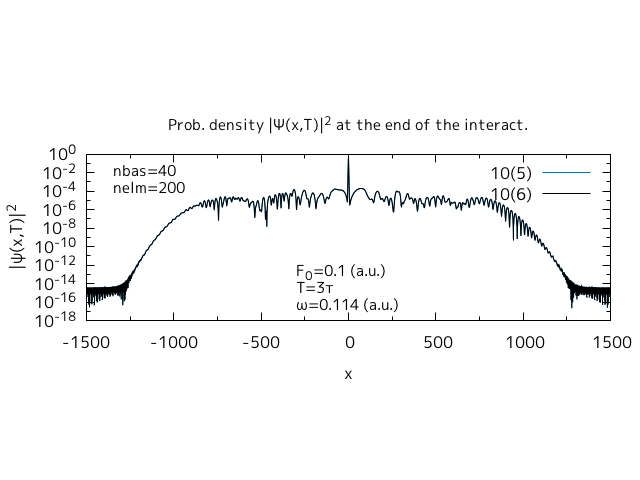
\includegraphics[scale=.20, trim={6 100 10 133},clip]{images/114_f01_3_density_comp.png} \\
% 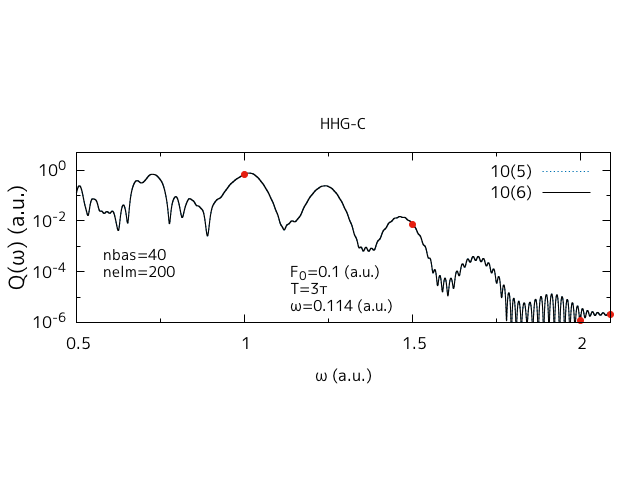
\includegraphics[scale=.20, trim={6 100 10 130},clip]{images/114_f01_3_hhg_comp.png} \\
%% \includegraphics[scale=.20, trim={6 130 10 130},clip]{images/114_f003_8_03_hhg.png} 
%%%\caption{Eigenvalues.}
%%\label{fig:pemd_0114}
% \end{figure}
%
%\end{minipage}
%\end{textblock*}
%
%
%\begin{textblock*}{500pt}(130pt,60pt)
%%\centering
%%\rotatebox{90}{
% \begin{minipage}{0.0\linewidth}
% \begin{figure}[tp]
% 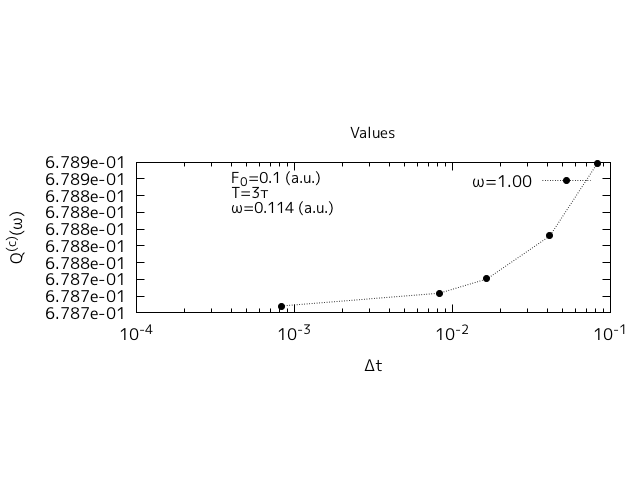
\includegraphics[scale=.20, trim={6 100 10 133},clip]{images/114_f01_3_values_100.png} \\
% 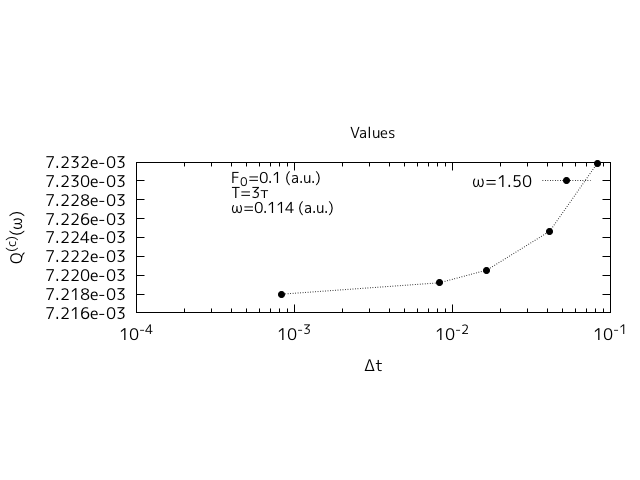
\includegraphics[scale=.20, trim={6 100 10 130},clip]{images/114_f01_3_values_150.png} \\
%% 
\includegraphics[scale=.20, trim={30 130 10 130},clip]{images/114_f003_12_07_hhg.png} 
%%%\caption{Eigenvalues.}
%%\label{fig:pemd_0114}
% \end{figure}
%
%\end{minipage}
%\end{textblock*}
%
%
%\begin{textblock*}{500pt}(255pt,60pt)
%%\centering
%%\rotatebox{90}{
% \begin{minipage}{0.0\linewidth}
% \begin{figure}[tp]
% 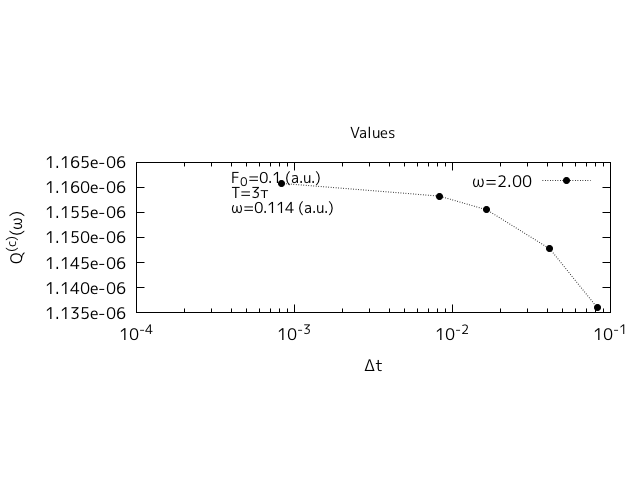
\includegraphics[scale=.20, trim={6 100 10 133},clip]{images/114_f01_3_values_200.png} \\
% 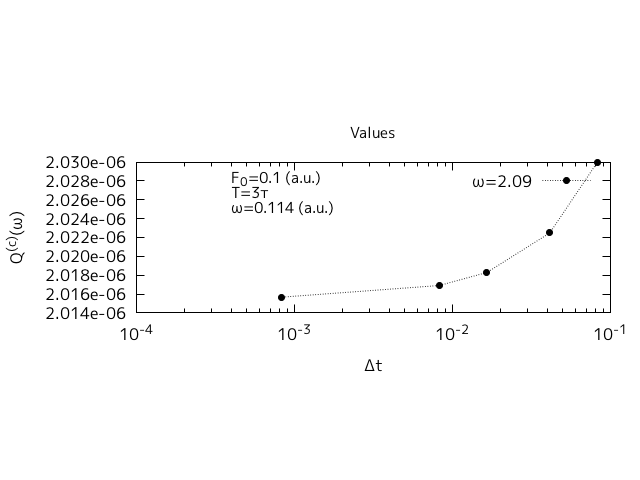
\includegraphics[scale=.20, trim={6 100 10 130},clip]{images/114_f01_3_values_209.png} \\
%% 
\includegraphics[scale=.20, trim={30 130 10 130},clip]{images/114_f003_12_07_hhg.png} 
%%%\caption{Eigenvalues.}
%%\label{fig:pemd_0114}
% \end{figure}
%
%\end{minipage}
%\end{textblock*}
%
%
%\begin{textblock*}{500pt}(390pt,165pt)
%%\centering
%\rotatebox{90}{
% \begin{minipage}{0.0\linewidth}
% \begin{figure}[tp]
% 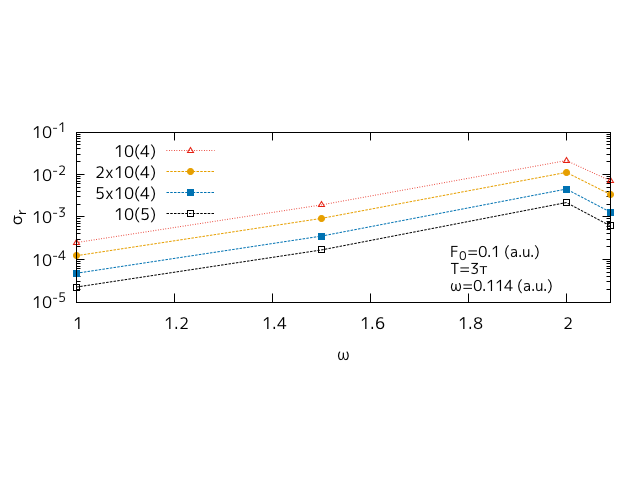
\includegraphics[scale=.20, trim={6 100 10 120},clip]{images/114_f01_3_error.png } \\
%%%\caption{Eigenvalues.}
%%\label{fig:pemd_0114}
% \end{figure}
%\end{minipage}
%}
%\end{textblock*}
%
%
%
%
%\begin{textblock*}{\linewidth}(20pt,170pt)
%\rotatebox{0}{
%\begin{minipage}{\linewidth}
%{
%\tiny 
%\centering
%\input{tables/114_f01_3t_error_2.tab}
%}
%\end{minipage}
%}
%\end{textblock*}
%
%
%\begin{textblock*}{400pt}(30pt,205pt)
%\scriptsize
%
%\begin{align}
%    \sigma_{ij}= \left|\frac{\left(   Q^{(c)}(\omega)[i] 
%       - Q^{(c)}(\omega)[j]  \right)}{Q^{(c)}(\omega)[j]}\right|, \hspace{20pt}
%    Q^{(c)}(\omega) & = \left|\Bigg[ e^{i\omega t} x(t)\Bigg]_{-T/2}^{T/2}
%               -i\omega \int_{-T/2}^{T/2} e^{i\omega t}x(t)dt\right|^2.
%                \nonumber
%\end{align}
%
%\end{textblock*}
%
%\end{frame}
%
%
%
%
%
%
%\begin{frame}
%\frametitle{Quantum theory of radiation by nonstationary systems 
%	with application to high-order harmonic generation
%        (Phys. Rev. A 101, 013410 (2020))}
%	\framesubtitle{Time dependence - $T=8\tau$}
%\small
%\begin{textblock*}{500pt}(5pt,60pt)
%%\centering
%%\rotatebox{90}{
% \begin{minipage}{0.0\linewidth}
% \begin{figure}[tp]
% 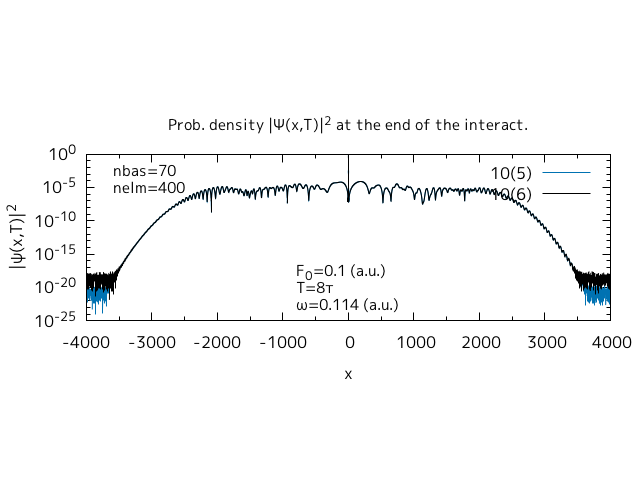
\includegraphics[scale=.20, trim={6 100 10 133},clip]{images/114_f01_8_density_comp.png} \\
% 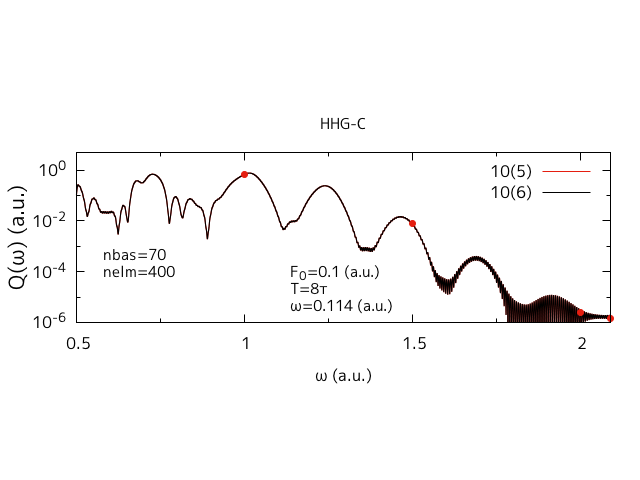
\includegraphics[scale=.20, trim={6 100 10 130},clip]{images/114_f01_8_hhg_comp.png} \\
%% \includegraphics[scale=.20, trim={6 130 10 130},clip]{images/114_f003_8_03_hhg.png} 
%%%\caption{Eigenvalues.}
%%\label{fig:pemd_0114}
% \end{figure}
%
%\end{minipage}
%\end{textblock*}
%
%
%\begin{textblock*}{500pt}(130pt,60pt)
%%\centering
%%\rotatebox{90}{
% \begin{minipage}{0.0\linewidth}
% \begin{figure}[tp]
% 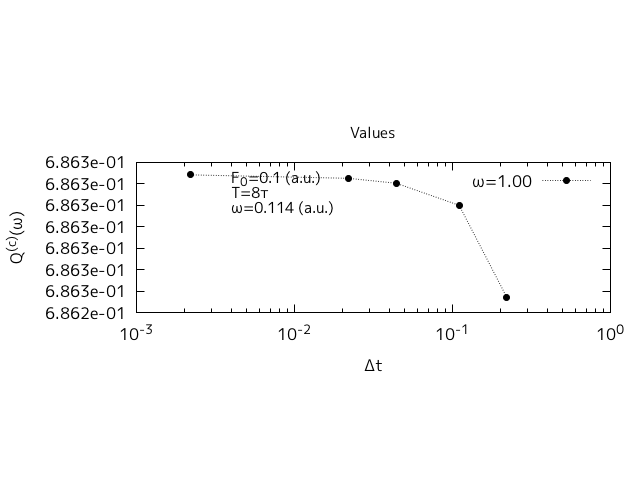
\includegraphics[scale=.20, trim={6 100 10 133},clip]{images/114_f01_8_values_100.png} \\
% 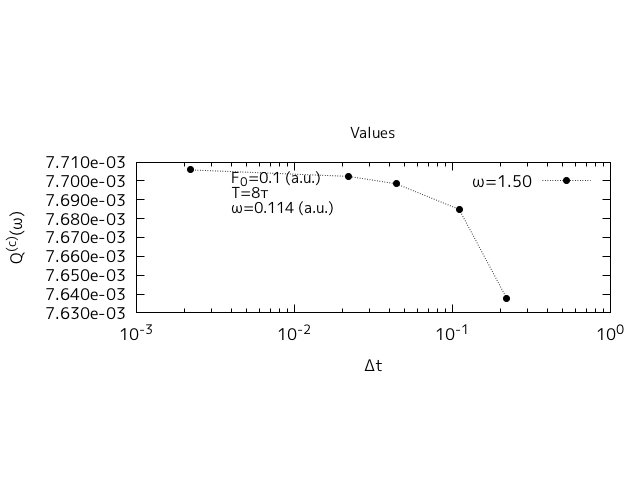
\includegraphics[scale=.20, trim={6 100 10 130},clip]{images/114_f01_8_values_150.png} \\
%% 
\includegraphics[scale=.20, trim={30 130 10 130},clip]{images/114_f003_12_07_hhg.png} 
%%%\caption{Eigenvalues.}
%%\label{fig:pemd_0114}
% \end{figure}
%
%\end{minipage}
%\end{textblock*}
%
%
%\begin{textblock*}{500pt}(255pt,60pt)
%%\centering
%%\rotatebox{90}{
% \begin{minipage}{0.0\linewidth}
% \begin{figure}[tp]
% 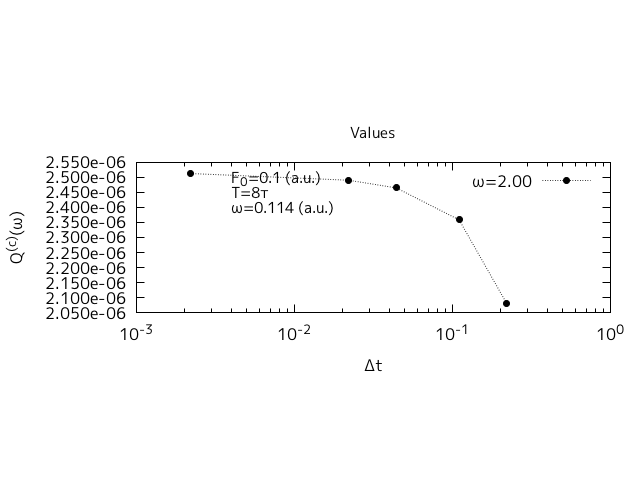
\includegraphics[scale=.20, trim={6 100 10 133},clip]{images/114_f01_8_values_200.png} \\
% 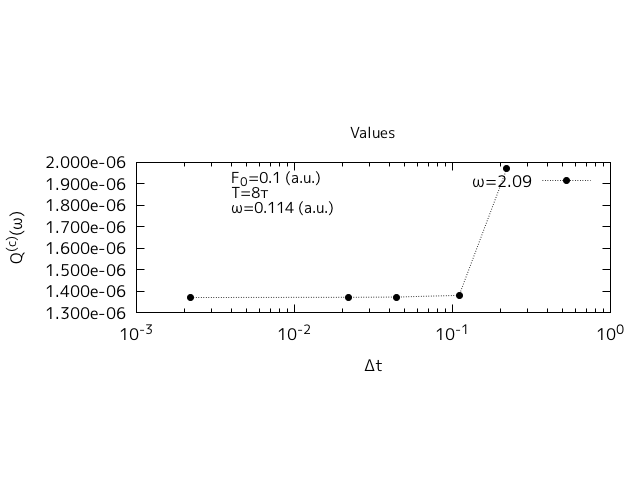
\includegraphics[scale=.20, trim={6 100 10 130},clip]{images/114_f01_8_values_209.png} \\
%% 
\includegraphics[scale=.20, trim={30 130 10 130},clip]{images/114_f003_12_07_hhg.png} 
%%%\caption{Eigenvalues.}
%%\label{fig:pemd_0114}
% \end{figure}
%
%\end{minipage}
%\end{textblock*}
%
%
%\begin{textblock*}{500pt}(390pt,165pt)
%%\centering
%\rotatebox{90}{
% \begin{minipage}{0.0\linewidth}
% \begin{figure}[tp]
% 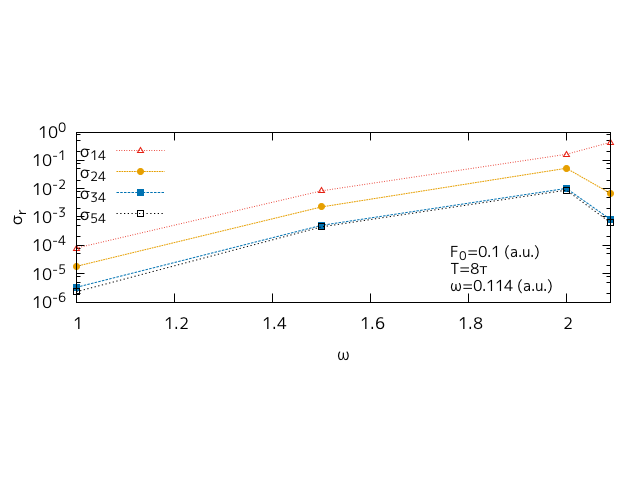
\includegraphics[scale=.20, trim={6 100 10 120},clip]{images/114_f01_8_error.png } \\
%%%\caption{Eigenvalues.}
%%\label{fig:pemd_0114}
% \end{figure}
%\end{minipage}
%}
%\end{textblock*}
%
%
%
%
%\begin{textblock*}{\linewidth}(20pt,170pt)
%\rotatebox{0}{
%\begin{minipage}{\linewidth}
%{
%\tiny 
%\centering
%\input{tables/114_f01_8t_error_2.tab}
%}
%\end{minipage}
%}
%\end{textblock*}
%
%
%\begin{textblock*}{400pt}(30pt,205pt)
%\scriptsize
%
%\begin{align}
%    \sigma_{ij} = \left|\frac{\left(   Q^{(c)}(\omega)[i] 
%       - Q^{(c)}(\omega) [j] \right)}{Q^{(c)}(\omega)[j]}\right|, \hspace{20pt}
%    Q^{(c)}(\omega) & = \left|\Bigg[ e^{i\omega t} x(t)\Bigg]_{-T/2}^{T/2}
%               -i\omega \int_{-T/2}^{T/2} e^{i\omega t}x(t)dt\right|^2.
%                \nonumber
%\end{align}
%
%\end{textblock*}
%
%\end{frame}



\begin{frame}
\frametitle{Quantum theory of radiation by nonstationary systems 
	with application to high-order harmonic generation
        (Phys. Rev. A 101, 013410 (2020))}
	\framesubtitle{Time dependence reference table - (homogeneous problem)}
\small

\begin{textblock*}{400pt}(30pt,60pt)
\footnotesize
\begin{itemize}
\item Sufficient time step for converged result is 
$\Delta t \leqslant 0.08\,\rm a.u.$
\item In the following, we will maintain $\Delta t$ set to 
around $0.04\,\rm a.u.$
\end{itemize}


	\textcolor{red}{\textbf{Those are old data. Just a reminder}}\\

\end{textblock*}

{
\tiny 
\input{tables/ref_dt.tab}
}


\begin{textblock*}{400pt}(30pt,205pt)
\scriptsize

\begin{align}
    \tau = n_{oc}\frac{2\pi}{\omega}, \hspace{20pt}
    T = n \tau, \hspace{20pt}
    \Delta t  = \frac{T}{{\rm nsteps}}, \hspace{20pt}
    n_{oc}  = 5,
                \nonumber
\end{align}

\end{textblock*}

\end{frame}




\begin{frame}
\frametitle{Quantum theory of radiation by nonstationary systems 
	with application to high-order harmonic generation
        (Phys. Rev. A 101, 013410 (2020))}
	\framesubtitle{Convergence parameters table for 
             the homogeneous equation}
\small

\begin{textblock*}{400pt}(30pt,60pt)
\footnotesize
\begin{itemize}
\item The following table shows parameters known to return converged results 
for Eq. (\ref{eqn:step_1d}), which is recalled below
%\item \textbf{For $\omega=0.057\,\rm a.u.$ and $F_0 = 0.3\,\rm a.u.$,
%PEMD and HHG spectra currently do not converge even 
%when density probability does}
\end{itemize}
	\textcolor{red}{\textbf{Those are old data. Just a reminder}}\\
	\textcolor{red}{\textbf{What we want now, 
	is to extend this logic to the inhomogeneous case}}

\end{textblock*}

\vspace{20pt}

{
\tiny 
\input{tables/conv_table_057.tab}
\input{tables/conv_table_114.tab}
}


\begin{textblock*}{400pt}(30pt,205pt)
\scriptsize

\begin{equation}
	i\frac{\partial}{\partial t}\psi(x,t)
	   = \left( \hat{H}_a + \hat{V}_{\rm ext}(t)\right) 
	   \psi(x,t),   \hspace{20pt}\psi(x,0)=\psi_0(x), \nonumber
\end{equation}
\begin{equation}
  \hat{H}_a = -\frac{1}{2}\frac{d^2}{dx^2} - \varkappa\delta(x), \hspace{20pt}
  \hat{V}_{\rm ext} = F(t)x,   \nonumber
\end{equation}

\end{textblock*}


\begin{textblock*}{100pt}(30pt,140pt)
\scriptsize
\textbf{Legend} \\
$\rm (nbas/nelm) - xmax $


\end{textblock*}

\end{frame}

